\section{Introduction} \label{sec:intro}
The discovery of the binary neutron star merger GW170817
\citep{TheLIGOScientific:2017qsa} has given us a new way to explore the
physics of neutron stars. Recent studies have measured the star's tidal
deformability and placed constraints on the equation of state of the neutron
stars~\citep{TheLIGOScientific:2017qsa,Tews:2018iwm,Most:2018eaw,Raithel:2018ncd,de2018tidal,Abbott:2018exr,Abbott:2018wiz}.
\cite{Weinberg:2013pbi} have suggested that the star's tidal deformation can
induce nonresonant and nonlinear daughter wave excitations in $p$- and
$g$-modes of the neutron stars via a quasi-static instability. This
instability would remove energy from a binary system and possibly affect the
phase evolution of the gravitational waves radiated during the inspiral.
Although \cite{Venumadhav:2013nla} concluded that there is no quasi-static
instability and hence no effect on the inspiral, \cite{Weinberg:2015pxa}
claims that the instability can rapidly drive modes to significant energies
well before the binary merges. However, the details of the instability
saturation are unknown and so the size of the effect of the $p$-$g$ mode
coupling on the gravitational-waveform is not known~\citep{Weinberg:2015pxa}.
The discovery of the binary neutron star merger GW170817 by Advanced LIGO and
Virgo provides an opportunity to determine if there is evidence for nonlinear
tides from $p$-$g$ mode coupling during the binary inspiral. 

Since the physics of the $p$-$g$ mode instability is uncertain,
\cite{Essick:2016tkn} developed a parameterized model of the energy loss due
to nonlinear tides. This model is parameterized by the amplitude and the
frequency dependence of the energy loss, and the gravitational-wave frequency
at which the instability saturates and the energy loss turns on. For plausible
assumptions about the saturation, \cite{Essick:2016tkn} concluded that $>
70\%$ of binary merger signals could be missed if only point-particle
waveforms are used, and that nonlinear tides may significantly bias the
measured parameters of the binary. Bayesian inference can be used to place
constraints on nonlinear tides during the inspiral of GW170817. An analysis by
\cite{abbott2019constraining} found that the GW170817 signal is consistent with both
a model that neglects the energy loss due to nonlinear tides and a broad range
of the $p$-$g$ mode parameters.  \cite{abbott2019constraining} constrain the
phenomenolgical amplitude parameter of the  nonlinear tides to $A < 10^{-7}$
at the 90\% credible interval. 

In this paper, we investigate the measurability of non-linear tides using the
GW170817 signal. We consider two models of the gravitational waves radiated
during the inspiral of GW170817. The first model is that used by
\cite{de2018tidal} to measure the tidal deformability and radii of the neutron
stars. Using the parameterized energy loss due to nonlinear tides given by
~\cite{Essick:2016tkn}, we construct a second model that includes the
leading order effect of the $p$-$g$ mode coupling on the wave's phasing.  The
PyCBC Inference package~\citep{alex_nitz_2018_1208115,biwer2019pycbc} is used
to calculate Bayes factors comparing these models, hence determining if either
hypothesis is preferred by the observation.  We first consider a model with a
weak constraint on the measurability of the non-linear tides: we require the
effect of the $p$-$g$ mode instability causes a gravitational-wave phase shift
of at least $0.1$~rad from the time at which the inspiral signal enters the
detector's sensitive band to the time at which the compact objects merge.
Comparing these two models using the GW170817 data finds a Bayes factor of
order unity. Neither model is preferred by the data, consistent with the result
of \cite{abbott2019constraining}. 

We then compare waveforms that include $p$-$g$ mode effects to the standard
model to determine which regions of the $p$-$g$ mode parameter space are
measurable by the LIGO-Virgo network.  We use the maximum
mismatch~\cite{Apostolatos:1995pj} between the $p$-$g$ mode signals and the
standard waveform space as measure of detectability.  We find that a large
region of the $p$-$g$ mode parameter space is not measureable by the
LIGO-Virgo detectors, as either the nonlinear tide effect produces an effect
that is either too small to measure, or the effect enters the waveform in a
way that is degenerate with the other (non $p$-$g$ mode) intrinsic parameters
of the waveform. By resampling the posterior distributions of the $p$-$g$ mode
model with a measurability constraint, we compute the Bayes factor between the
two models as a function of measurability. We find that either the non-linear tides 
produce a phase shift too small to be measured, or their effect is degenerate
with the standard waveform parameters and hence it is not possible to claim
that they are present. Breaking this degeneracy is difficult, as
it would require measurement of the binary's chirp mass to a precision better
than the observed level of chirp mass skew $(\sim 0.005\, M_\odot)$
through a method that is \emph{independent} of the gravitational-wave observations.
Future work on the $p$-$g$ mode waveform dynamics may yield clearer results.

\section{Waveform model}
\label{sec:waveform}

As two neutron stars orbit each other, they lose orbital energy $E_\mathrm{orbital}$ due to gravitational radiation $\dot{E}_{GW}$. The gravitational waveform during the inspiral is well modeled by post-Newtonian theory~(see e.g. \cite{Blanchet:2013haa}).  The effect of the $p$-$g$ mode instability is to dissipate orbital energy by removing energy from the tidal bulge of the stars~\citep{Weinberg:2013pbi,Weinberg:2015pxa,Essick:2016tkn}. Once unstable, the coupled $p$- and $g$-modes are continuously driven by the tides, giving rise to an extra energy dissipation $\dot{E}_{NL}$ for each star in the standard energy-balance equation~\citep{Peters:1963ux} 
\begin{equation}
\dot{E}_\mathrm{orbital} = -\dot{E}_\mathrm{GW} - \dot{E}^1_\mathrm{NL} - \dot{E}^2_\mathrm{NL}.
\label{eqn:energy_bal}
\end{equation}
Since the details of how the nonlinear tides extract energy from the orbit is not known, \cite{Essick:2016tkn} constructed a simple model of the energy loss and calculated plausible values for the model's parameters. In this model, the rate of orbital energy lost during the inspiral is modified by 
\begin{equation}\label{eqn:energy_nl}
\dot{E}_\mathrm{NL} \propto A f^{n+2} \Theta (f - f_0),
\end{equation}
where $A$ is a dimensionless constant that determines the overall amplitude of the energy loss, $n$ determines the frequency dependence of the energy loss, and $f_0$ is the frequency at which the $p$-$g$ mode instability saturation occurs and the effect turns on. By solving Eq.~(\ref{eqn:energy_bal}), \cite{Essick:2016tkn} computed the leading order effect of the nonlinear tides on the gravitational-wave phase as a function of $A$, $n$, and $f_0$. In this analysis, they allowed each star to have independent values of $A$, $f_0$, and $n$, but found that the energy loss due to nonlinear tides depends relatively weakly on the binary's mass ratio. Hence, they consider a model that performs a Taylor expansion in the binary's component mass~\citep{DelPozzo:2013ala} and include only the leading order terms in the binary's phase evolution. Given this, we parameterize our nonlinear tide waveform with a single set of parameters $A$, $n$, and $f_0$, by setting $\dot{E}^1_\mathrm{NL} = \dot{E}^2_\mathrm{NL}$. We  keep only the leading order nonlinear tide terms when we obtain the quantities $t(f)$ and $\phi(f)$ used to compute the stationary phase approximation~\citep{Sathyaprakash:1991mt,Droz:1999qx,Lindblom:2008cm}. This approach is reasonable for GW170817, since both neutron stars have similar masses and radii~\citep{de2018tidal}.

The dependence of $A$, $n$, and $f_0$ on the star's physical parameters is not known~\citep{Weinberg:2015pxa}. \cite{Essick:2016tkn} estimate that plausible parameter ranges are $A \lesssim 10^{-6}$, $0 \lesssim n \lesssim 2$, and $30 \lesssim f_0 \lesssim 80$ Hz. \cite{Zhou:2018tvc} found that the frequency at which the instability begins to grow is equation-of-state dependent and can occur at gravitational-wave frequencies as high as $700$~Hz. \cite{Andersson:2017iav} suggest that the instability may only act during the late stages of inspiral, (above $300$~Hz), otherwise the large energy dissipation will cause the temperature of the neutron stars to be very large. 

In this paper, we compare two models for the gravitational waves radiated by GW170817. The first is the standard restricted stationary-phase approximation to the Fourier transform of the gravitational waveform $\tilde{h}(f)$, known as the TaylorF2 waveform~\citep{Sathyaprakash:1991mt}. We begin with the same waveform model used by \cite{de2018tidal}, which is accurate to 3.5 PN order in the orbital phase, 2.0 PN order in spin-spin, self-spin and quadrupole-monopole interactions, 3.5 PN order in spin-orbit coupling, and includes the leading and next-to-leading order corrections from the star's tidal deformability~\citep{Kidder:1992fr,Blanchet:1995ez,Blanchet:2004ek,Buonanno:2009zt,Arun:2008kb,Marsat:2013caa,Bohe:2013cla,Bohe:2015ana,Mikoczi:2005dn, Flanagan:2007ix,Vines:2011ud}. We then construct a second model that adds the leading order effect of nonlinear tides computed using the model of \cite{Essick:2016tkn}. We compute the Fourier phase for the TaylorF2 model $\Psi(f)_\mathrm{TaylorF2}$ and add a term that accounts for the additional energy lost due to nonlinear tides $\Psi_\mathrm{NL}(f)$, given by
\begin{equation}
\Psi_\mathrm{NL}(f) = - \frac{25}{768} A \left(\frac{G \mathcal{M} \pi f_\mathrm{ref}}{c^3} \right)^{-\frac{10}{3}} \times \left \{
                     \begin{array}{ll}
                       \left( \frac{f_0}{f_\mathrm{ref}} \right)^{n-3} \left[ \left( \frac{f}{f_0}\frac{1}{n-4} \right) - \frac{1}{n-3} \right] &\quad f < f_0, \\
                       \left( \frac{f}{f_\mathrm{ref}} \right)^{n-3} \left(\frac{1}{n-4} - \frac{1}{n-3} \right)  &\quad f \ge f_0.
                     \end{array}
                     \right.
\label{eqn:fourier_phase_eq1}
\end{equation}
Here, $f_\mathrm{ref}$ is a reference frequency which we set to $100$~Hz following \cite{Essick:2016tkn}, $G$ is Newton's gravitational constant, $c$ is the speed of light, and $\mathcal{M} = (m_1 m_2)^{3/5}/(m_1+m_2)^{1/5}$ is the chirp mass of the binary.\footnote{Appendix~A of \cite{Essick:2016tkn} gives the change to the gravitational-wave phase $\phi(f)$ as a function of frequency and not the change to the Fourier phase $\Psi(f)$ (see e.g. \cite{Lindblom:2008cm} for a discussion of how these differ). The former quantity is useful to compute the change in the number of gravitational-wave cycles, but the latter is required to compute the modification to the TaylorF2 waveform.} We generate the standard TaylorF2 waveform using the LIGO Algorithm Library~\citep{lal} and multiply this frequency-domain waveform by the term due to the nonlinear tides,
\begin{equation}
\tilde{h}_\mathrm{TaylorF2+NL}(f) = \tilde{h}_\mathrm{TaylorF2}(f) \times \exp[-i \Psi_\mathrm{NL}(f) ].
\end{equation}
The Fourier phase for the nonlinear tides is implemented as a patch to the version of the PyCBC software~\citep{alex_nitz_2018_1208115} used by~\cite{de2018tidal}. Both the standard and nonlinear tide waveform models are terminated when the gravitational-wave frequency reaches that of a test particle at the innermost stable circular orbit of a Schwarszchild black hole of mass $M = m_1 + m_2$. For the neutron star masses considered here, this frequency is between 1.4 kHz and 1.6 kHz.

There are however, some challenges with using this waveform model to measure the parameters of a gravitational wave signal. Of particular note, this waveform model permits a degeneracy in the signal morphology with chirp mass. When $n = 4/3$, the Fourier phase in Eq.~(\ref{eqn:fourier_phase_eq1}) for nonlinear tides gives $\Psi(f) \propto f^{-5/3}$, which is the same power law dependence as the chirp mass phasing. This degeneracy is exacerbated in waveform modeling when the amplitude $A$ is large and when $f_0$ is low. If $f_0$ is comparable or lower than the frequency at which chirp mass can be accurately measured it is possible to match to the standard general relativity point-particle waveform with a smaller chirp mass than would be measured without the nonlinear tidal phasing terms. In principle, there will be other degeneracies with other intrinsic parameters of the gravitational wave signal for other values of $n$.

\section{Model Priors} \label{sec:priors}
Bayes theorem offers a methodology for evaluating the plausibility of models relative to a given data set, and then updating these prior model beliefs with better hypotheses. Bayes theorem states that
\begin{equation}
p\left(\vec{\theta}\,| H, \mathbf{d}\right) = \frac{ p\left(\mathbf{d}|H, \vec{\theta}\,\right)\, p\left(\vec{\theta}\,|H\right)}{p\left(\mathbf{d}|H\right)},
\label{eq:bayestheorem}
\end{equation}
where $p \left(\mathbf{d}|H \right)$ is the evidence of the model $H$, $p\left(\vec{\theta}\,|H\right)$ is the is the prior distribution of the parameters given the signal model, $p\left(\mathbf{d}|H, \vec{\theta}\right)$ is the likelihood of the data for a particular set of parameters $\vec{\theta}$, and $p\left( \vec{\theta}\,|H, \mathbf{d}\right)$ is the posterior distribution of the parameters given the signal model. The likelihood used in this analysis assumes a Gaussian model of detector noise and depends upon the noise-weighted inner product between the gravitational waveform and the data from the gravitational-wave detectors~\citep{Finn:2000hj,Rover:2006bb}. The choice of prior distributions on the parameters of the signal model represent the hypothesis that we want to test. The posterior distributions reflect how to update ones beliefs with respect to the likelihood and the data. Thus, by examining many different parameter hypotheses we can investigate the extent to which GW170817 is accurately modeled by $p$-$g$ mode instability waveform models.

In our analysis, We fix the sky location and distance to GW170817~\citep{Soares-Santos:2017lru,Cantiello:2018ffy} and assume that both neutron stars have the same equation of state by imposing the common radius constraint~\citep{de2018tidal}. In the case of the standard TaylorF2 waveform $H_\mathrm{TaylorF2}$, our analysis is identical to that described in~\cite{de2018tidal}. This analysis considered three prior distributions on the binary's component mass. Here, we only consider the uniform prior on each star's mass, with $m_{1,2} \sim U[1,2]\, M_\odot$, and the Gaussian prior on the component masses $m_{1,2} \sim N(\mu = 1.33, \sigma = 0.09)\, M_\odot$~\citep{Ozel:2016oaf}. For both mass priors, we restrict the chirp mass to the range $ 1.1876 M_\odot < \mathcal{M} < 1.2076 M_\odot$. Since our analysis is identical to that of~\citep{de2018tidal}, we refer to that paper for the details of the data analysis configuration.

Given the uncertainty on the range of the nonlinear tide parameters, we draw $n \in U[-1.1, 2.999]$, and $A$ from a distribution uniform in $\log_{10}$ between $10^{-10}$ and $10^{-6}$. We investigate two choices of drawing $f_0$: we draw $f_0$ from a uniform distribution between $15$ and $100$~Hz, as used by~\cite{Essick:2016tkn}, and from a uniform distribution between $15$ and $800$~Hz to allow for the larger values of $f_0$ suggested by~\cite{Zhou:2018tvc} and~\cite{Andersson:2017iav}.

Since some combinations of $A$, $n$, and $f_0$ can produce extremely small gravitational-wave phase shifts~\citep{Essick:2016tkn}, we place a cut on the gravitational-wave phase shift due to nonlinear tides
\begin{equation}
\delta \phi(f_\mathrm{ISCO}) =
                      \frac{-25}{768}  \frac{A}{n-3} \left( \frac{G \mathcal{M} \pi f_{ref}}{c^3} \right)^{-10/3} \left[ \left( \frac{f_0}{f_{ref}} \right)^{n-3} - \left(\frac{f_\mathrm{ISCO}}{f_{ref}} \right)^{n-3} \right],
\end{equation}
where $f_\mathrm{ISCO}$ is the termination frequency of the waveform (which is always larger than $f_0$ in our analysis). This gravitational-wave phase shift from the $p$-$g$ mode instability is strictly negative, but we take the convention of using the absolute value of the phase shift for convenience. We restrict the prior space to values of $\delta \phi > 0.1$~rad. Phase shifts of $\delta \phi \approx 0.1$~rad have matches between the two waveform models greater than 99.98\%. This cut means that the resulting priors on $A$, $n$, and $f_0$ are not uniform, but are biased in favor of combinations of parameters that may produce a measurable effect due to nonlinear tides. While $\delta \phi$ is a simple proxy for how similar or dissimilar two waveforms are, formally this is given by the match between two waveforms. A $\delta \phi$ of $1$ radian may have a low overlap with a waveform if the radian is accumulated over a large bandwidth but a high overlap if the radian is accumulated near the very end of the signal.

We also explore a prior distribution on the nonlinear tidal parameters that closely following those found in ~\cite{abbott2019constraining}. Here we use $n \in U[-1.0, 2.999]$, $A$ from a distribution uniform in $\log_{10}$ between $10^{-10}$ and $10^{-5.5}$, and $f_0 \in U[10, 100]$~Hz. We place no constraint on the permissible gravitational-wave phase shift, permitting the prior model space to explore $\delta \phi \gtrsim 0.001$~rad of change at merger,  $f_\mathrm{ISCO}$. Fig.~\ref{fig:priors} shows a depiction of the prior distributions used in this study.

\begin{figure}[th]
\centering
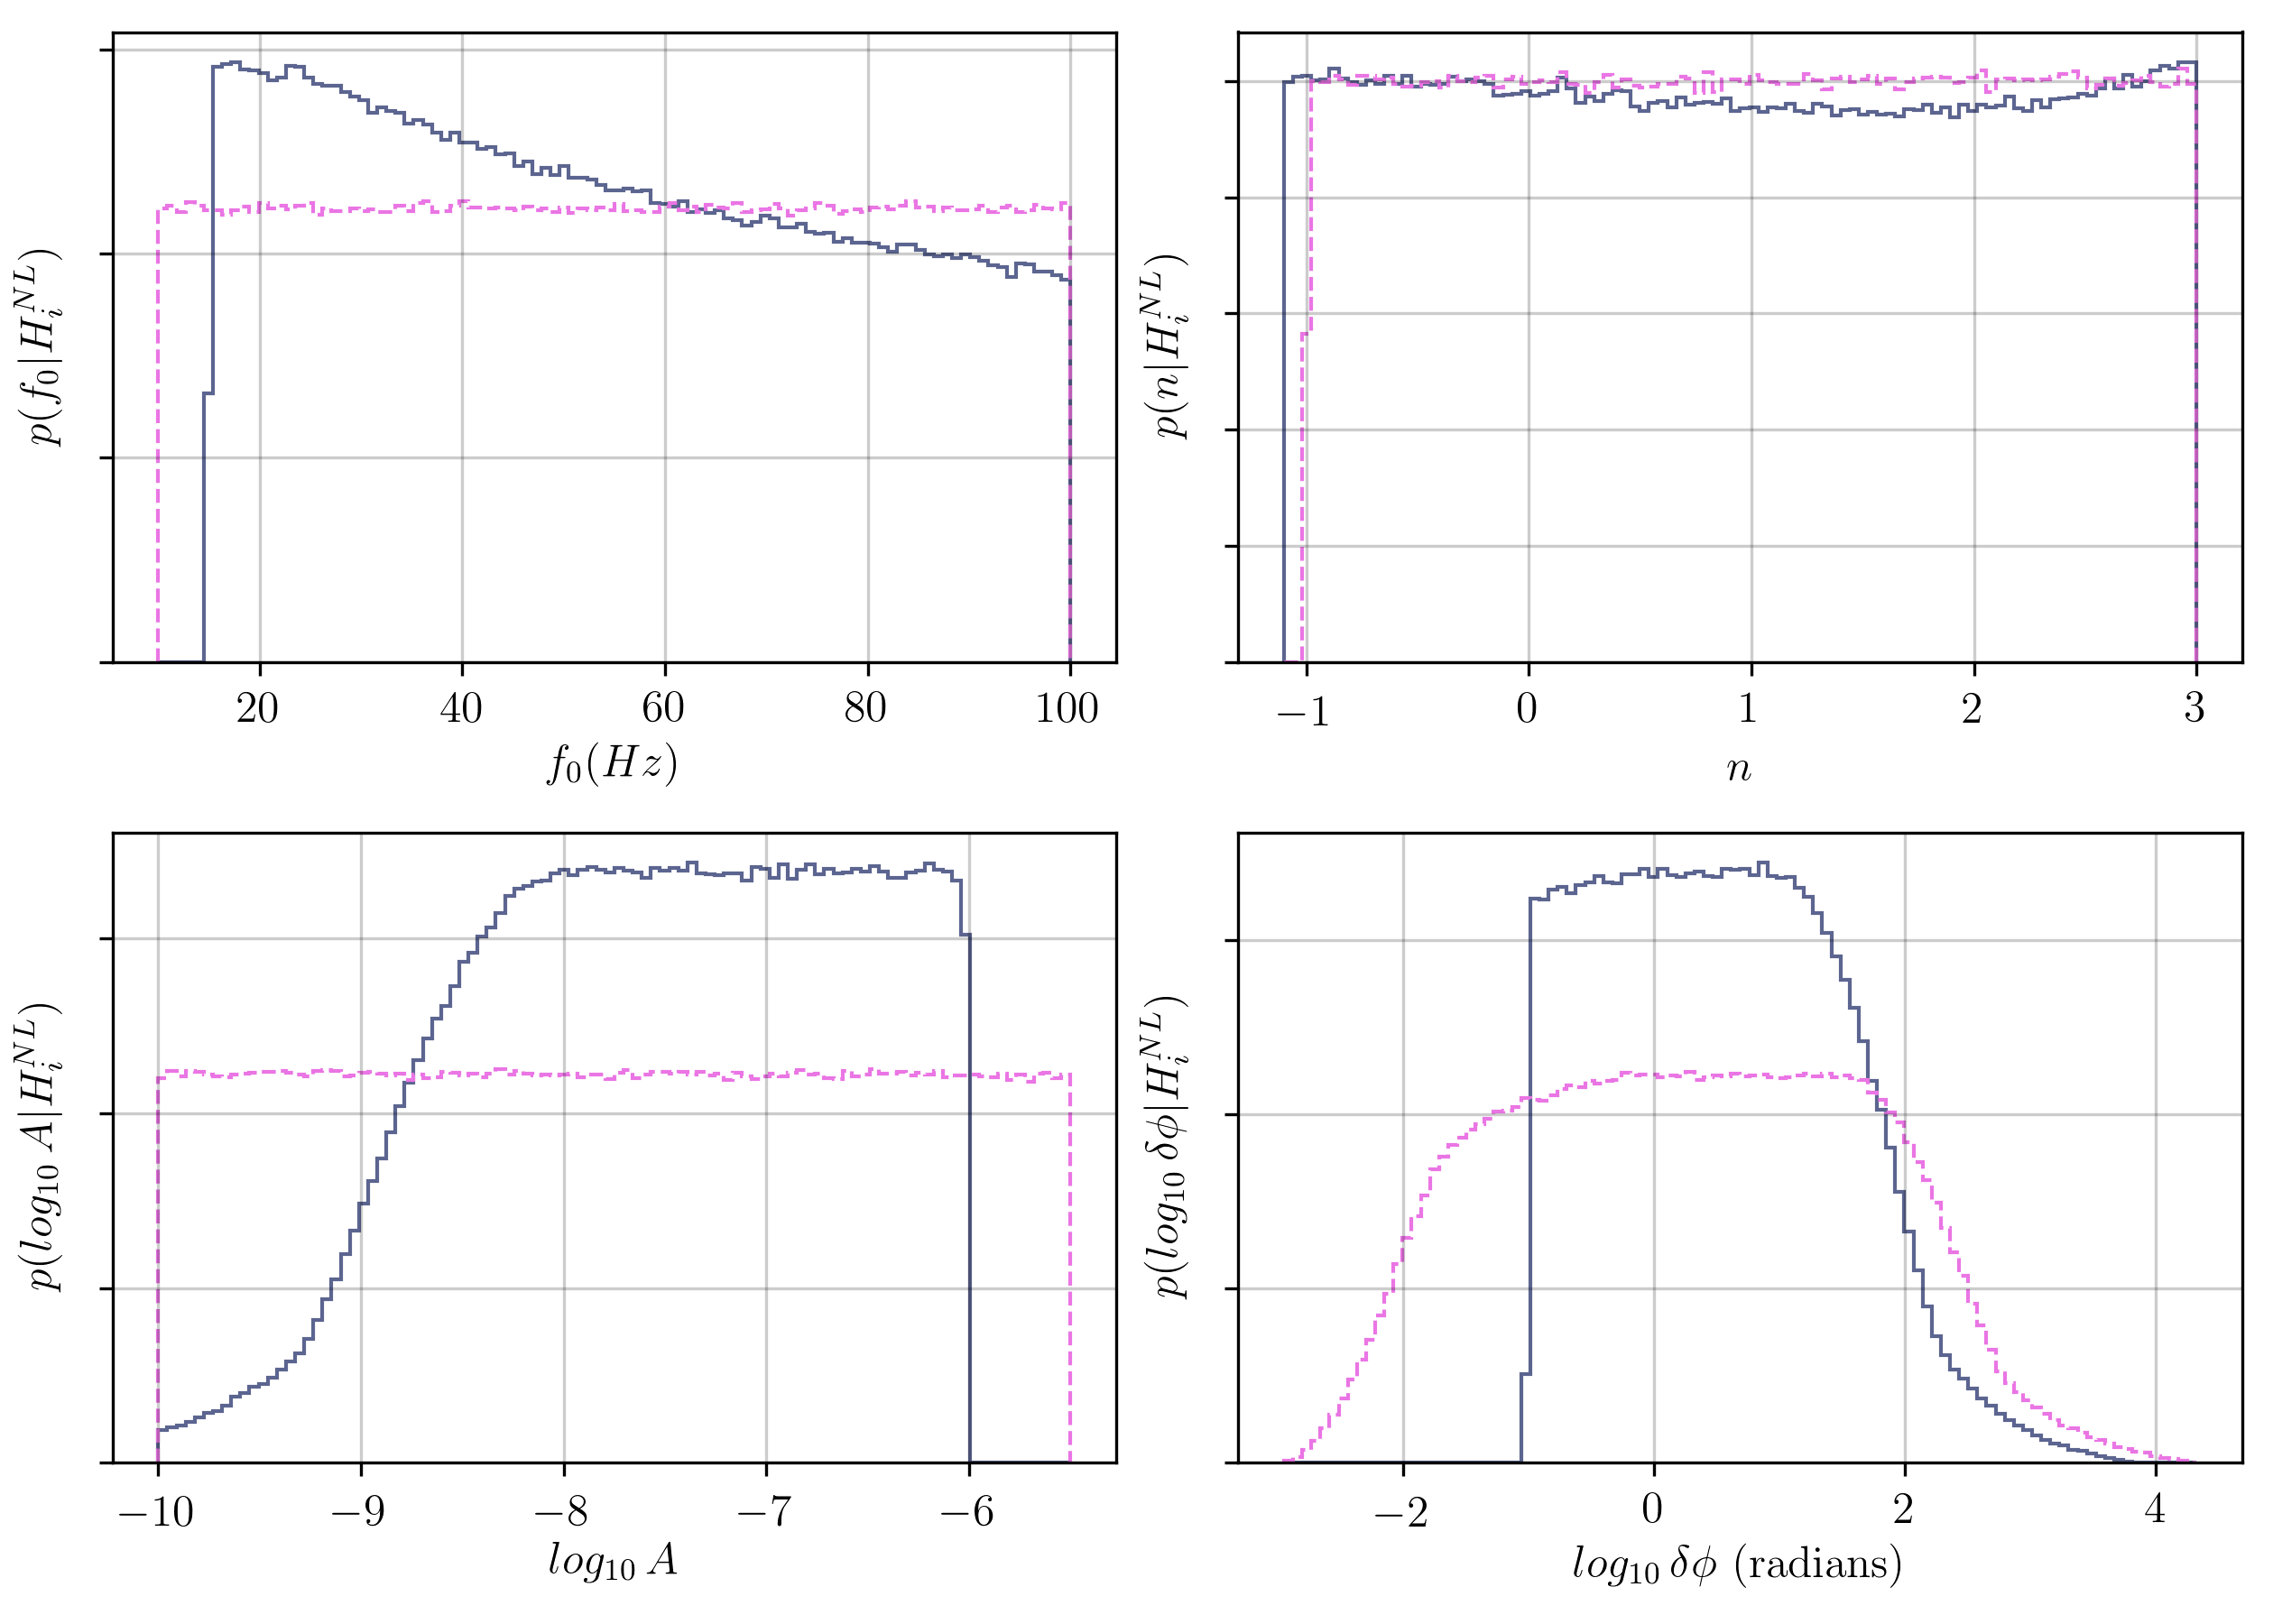
\includegraphics[width=0.9\columnwidth]{all_pg_priors.pdf}
\caption{Prior probability distributions on the parameters $(f_0, n, A)$ for the waveform model $H^{NL}_i = H_\mathrm{TaylorF2+NL}$ and the resulting prior on the gravitational-wave phase shift $\delta\phi$ shift due to nonlinear tides. The dark blue, solid lines shows the priors when $f_0$ is drawn from a uniform distribution between $15$ and $100$~Hz with a $\delta\phi \ge 0.1$~rad constraint restricting some of the prior space. The pink, dotted lines represent prior distributions on the nonlinear tidal parameters similar to~\cite{abbott2019constraining}.}
\label{fig:priors}
\end{figure}

A stricter approach to constructing a prior distribution is to examine the maximum overlap between a distribution of $p$-$g$ mode waveform and a set of comparable TaylorF2 waveforms. At the moment it is computationally expensive to conduct hypothesis testing with a prior drawn from a highly correlated parameter space such as this. However, it is instructive to examine the results of a Bayesian inference with respect to a template bank of non-spinning, mass-only TaylorF2 waveforms. To do so we construct a template bank of $\sim 20,000$ non-spinning, mass-only template bank of comparable masses to the prior distribution on the mass parameters. The template bank is constructed with component masses, $m_{(1,2)} \in (1.0, 2.0) M_{\odot}$, chirp masses, $\mathcal{M}_c \in (1.1826, 1.2126) M_{\odot}$, and a minimal match placement of 99.9\%. When we examine the fitting factor between nonlinear tidal waveforms and this template bank we observe that there is a very high match between standard templates and nonlinear tidal waveforms when $n = 4/3$. The nonlinear tidal waveforms that least match this template bank tend to be those parameterized by large amplitude and large gravitational-wave phase shift.

\section{Methods} \label{sec:methods}
We use the gravitational-wave strain data from the Advanced LIGO and Virgo detectors for the GW170817 event, made available through the LIGO Open Science Center~\citep{Vallisneri:2014vxa,gw170817-losc}.

We then repeat the analysis of~\cite{de2018tidal} using the waveform model $H_\mathrm{TaylorF2+NL}$ to compute the evidence $p(\mathbf{d}|H_\mathrm{TaylorF2+NL})$.
The PyCBC Inference package~\citep{alex_nitz_2018_1208115,biwer2019pycbc} is used
to calculate Bayes factors comparing these models, hence determining which
hypothesis is supported by the observations. 

We use Bayesian model selection to determine which of the two waveform models described in Sec.~\ref{sec:waveform} is better supported by the observations of GW170817. Bayes theorem in Eq.~(\ref{eq:bayestheorem}) permits us a method for model  through the ratio of the evidence from each model. This ratio of the model evidences is called the Bayes factor, which we denote as $\mathcal{B}$. A Bayes factor greater than unity indicates support for the model in the numerator, while a Bayes factor less than unity indicates support for the model in the denominator. The Bayes factor can be written as,
\begin{equation}
\mathcal{B} = \frac{p\left(\mathbf{d}|H_\mathrm{TaylorF2+NL}\right)}{p\left(\mathbf{d}|H_\mathrm{TaylorF2}\right)}.
\label{eq:bayesfactor}
\end{equation}
The numerator of Eq.~(\ref{eq:bayesfactor}) is the evidence for nonlinear tides $p\left(\mathbf{d}|H_\mathrm{TaylorF2+NL}\right)$. For the denominator of Eq.~(\ref{eq:bayesfactor}), we use the evidence $p(\mathbf{d}|H_\mathrm{TaylorF2})$ provided as supplemental materials by~\citep{de2018tidal}.

Posterior distributions for parameters of interest can be also computed by marginalizing the posterior probability distribution over other parameters.  Marginalization to obtain the posterior probabilities and the evidence is performed using Markov Chain Monte Carlo (MCMC) techniques. To compute posterior probability distributions and evidences, we use the \emph{PyCBC Inference} software~\citep{alex_nitz_2018_1208115,biwer2019pycbc} using the the parallel-tempered \emph{emcee} sampler~\citep{emcee,vousden:2016}.
This sampler allows the use of multiple temperatures to sample the parameter space~\citep{emcee, doi:10.1143/PTPS.157.317, B509983H}.

From these multiple temperatures we use the thermodynamic integration method~\citep{lartillot2006computing,friel2008marginal} to estimate the logarithm of the evidence, ln $z$, given as:
\begin{equation}
\textrm{ln} \, z = \int_0^1 \langle \textrm{ln} \, \mathcal{L} \rangle_{\beta} \, d\beta
\label{eq:thermoint}
\end{equation}
The estimate of the evidence is determined by the integral over inverse temperatures, $\beta$, of the average log likelihood, $\langle \textrm{ln}\, \mathcal{L} \rangle_{\beta}$, for each inverse temperature $\beta$. An approximation to this integral can be made through use of trapezoid rule integration method. Following~\cite{de2018tidal} we use $51$ temperatures where we use a combination of geometric and logarithmic temperature placements to improve the accuracy of the integral~\citep{liu2016evaluating}.

We verify the results of the thermodynamic integration evidence calculation by comparing it with the steppingstone algorithm~\citep{xie2010improving}, which utilizes the same log likelihoods from multi-tempering sampling as the thermodynamic integration method. Both trapezoidal rule thermodynamic integration and steppingstone methods can have some bias in the estimate of the logarithm of the evidence due to a finite number of temperatures being used. This bias is mitigated by an increased number of temperatures~\citep{xie2010improving, Russel:2018pqv} and we believe it to be very small in this study.

We also estimate the error for each method of evidence calculation. The thermodynamic integration method and steppingstone algorithm both contain Monte Carlo error~\citep{annis2019thermodynamic}. For the thermodynamic integration method the Monte Carlo error is an estimate of the variance of the average log likelihood at each temperature. This can be calculated following the methodology of~\cite{annis2019thermodynamic} to give a confidence interval on the Monte Carlo error of the thermodynamic integration under trapezoid rule. In~\cite{xie2010improving} there is a Monte Carlo variance estimate on the logarithm of the evidence that we use here.

The thermodynamic integration method under trapezoid rule can also be corrected for discretization error in the integration method by going to the next order of the trapezoidal rule integration~\citep{friel2014improving}. We will call this next order estimation the corrected trapezoid rule for thermodynamic integration. Following~\cite{annis2019thermodynamic}, we consider both the thermodynamic integration method with the trapezoid rule and corrected trapezoid rule as distinct estimators of the model evidence. We use the same Monte Carlo error for the simple trapezoid rule as for the corrected trapezoid rule.

The last source of error in the evidence calculation that we consider is whether the MCMC has converged to stable likelihood values across all of the temperatures. This requires examining the stability of the evidence calculations as the MCMC progresses. Independent samples are drawn according to the $\mathrm{n_{acl}}$ method as outlined by~\cite{biwer2019pycbc} at various points in the run. This method takes a specific endpoint iteration, takes half the endpoint iteration as the starting point iteration, and calculates the autocorrelation length of the samples between the starting point and the endpoint iteration. Independent samples are drawn in intervals of the maximum autocorrelation length for the samples within this segment. We divide the full run into $12$ segments and calculate the evidence from each one of these segments to examine how the evidence progresses along the MCMC iterations. Gradually the evidence begins to settle towards a constant value as the MCMC progresses. We take the difference between the last two evidence estimates as the convergence error.

We estimate the total error on our evidence calculations, $\sigma_{ln \, z}$, by adding the errors in quadrature according to,
\begin{equation}
\sigma_{ln \, z} = \sqrt{ \sigma_{\mathrm{MC}}^2 + \sigma_{\mathrm{convergence}}^2 } \, .
\label{eq:errorprop}
\end{equation}
Here, the error $\sigma_{MC}$ is the Monte Carlo error and $\sigma_{\mathrm{convergence}}$ is the convergence error. Finally, to estimate the Bayes factors we model the log evidence as a normal distribution, with mean given from the log evidence calculation, and standard deviation given by the error propagation formula in Eq.~(\ref{eq:errorprop}). The ratio of the log evidence samples drawn from these distributions then gives a distribution of plausible log Bayes factors for each model pair.

\section{Results}
\label{sec:results}
We find that in all cases, the Bayes factors for GW170817 cannot rule-in or rule-out the presence of nonlinear tides from $p$-$g$ mode coupling in GW170817. This is true independent of the mass prior distribution, or the range of $f_0$ considered. Following the Bayes factor metrics from~\cite{kass1995bayes, jeffreys1998theory}, these Bayes factors cannot be considered to be statistically significant. For the narrow range of $15 \le f_0 \le 100$~Hz where $\delta \phi > 0.1$~rad, we find that the Bayes factors are $\mathcal{B} \sim 0.6$. This is also true of the prior range $10 \le f_0 \le 100$~Hz with unconstrained $\delta \phi$. The broader range  $15 \le f_0 \le 800$~Hz, where $\delta \phi > 0.1$~rad, we find that $\mathcal{B} \sim 0.6$ as well. Our estimated statistical error on Bayes factors due to Monte Carlo error and convergence error is relatively small, $\sim \pm 0.1$ at the $10$\% and $90$\% confidence level.

When we consider the way that the nonlinear tides enter the Fourier phase in Eq.~(\ref{eqn:fourier_phase_eq1}), we see that if $n = 4/3$ then the nonlinear tides enter the Fourier phase of the waveform with the same power law dependence on frequency $f$ as the chirp mass, that is $\Psi(f) \propto f^{-5/3}$. We also note that for the effect of nonlinear tides to be degenerate with chirp mass, they must turn on at a frequency $f_0$ that is close to the low-frequency limit of the detector's sensitive band. If the effect turns on at higher frequencies, then the phasing will change in the detector's sensitive band and it is more difficult to compensate for the nonlinear tide effect with a change in chirp mass. 

Our results are consistent with this understanding of the phasing. The marginalized posteriors shown in Fig.~\ref{fig:uniform_f0_small} show a strong degeneracy between the source-frame chirp mass $\mathcal{M}^\textrm{src}$ and nonlinear tides that causes a second peak in the chirp mass posterior at lower values of chirp mass than the value measured using the standard waveform model, $\mathcal{M}^\textrm{src} = 1.1867\pm0.0001\, M_\odot$~\citep{de2018tidal}. We see a peak in the posteriors of $n$ and $f_0$ at $n \lesssim 4/3$ and $f_0 \lesssim 35$~Hz. These peaks are also correlated with large $A$, with $10^{-8} \lesssim A < 10^{-6}$. Since there are also degeneracies with the other intrinsic parameters the peaks are not exactly at the predicted values, but the chirp mass degeneracy is the leading order effect. The samples with large posterior values of $\delta\phi$ seen in Fig.~\ref{fig:uniform_f0_small} are strongly correlated with source-frame chirp masses $\mathcal{M}^\textrm{src} \lesssim 1.1866.$ We have examined the change to the posterior distribution when changing the low-frequency cutoff of the likelihood integration from $20$~Hz to $25$~Hz, and to $30$~Hz. In these analyses, the peak in the posterior of $f_0$ tracks the low-frequency cutoff of the likelihood integration, confirming that this effect is due to the chirp-mass degeneracy with the low-frequency cutoff.

The chirp mass degeneracy is still present in the analysis with the broader range of $f_0$, however it is not as pronounced in the posterior samples due to the larger prior space being explored.

\begin{figure}[th]
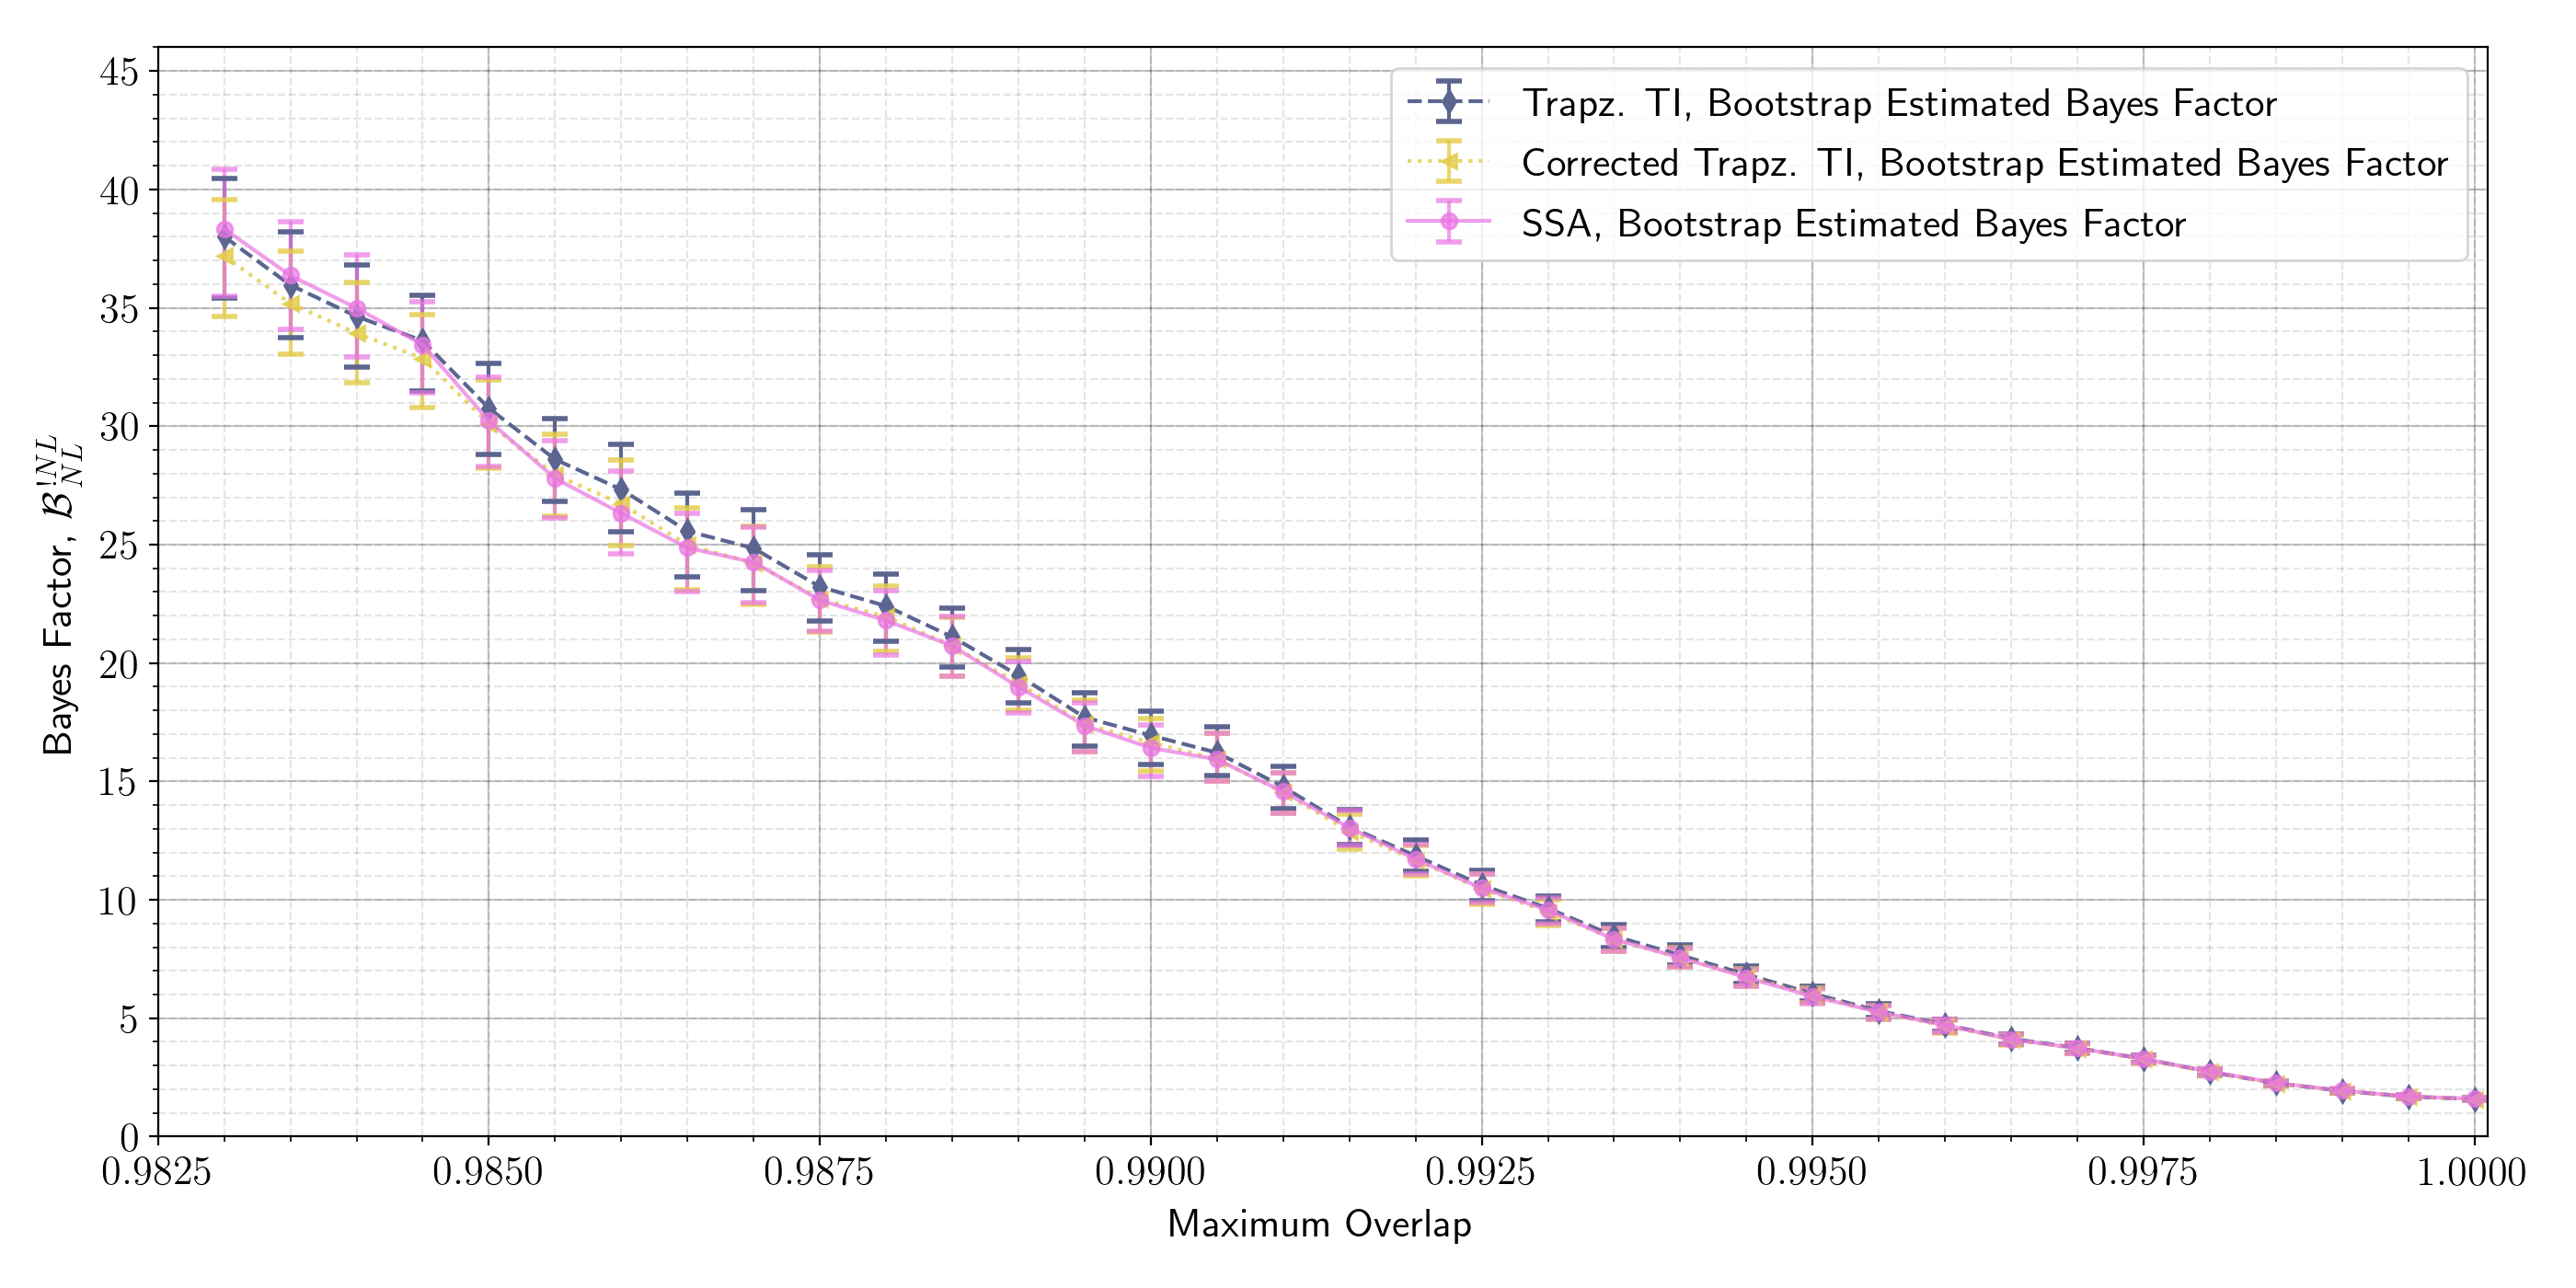
\includegraphics[width=\columnwidth]{bootstrap_bayes_ff_cuts_average}\caption{The projected Bayes factors for nonlinear tidal parameters when the samples from 9 runs are filtered by the fitting factor to a non-spinning, mass-only template bank of TaylorF2 waveforms. The convention in Bayes factor is switched from the main body of the text to represent the Bayes factor for the ratio of evidence for no nonlinear tides, $p\left(\mathbf{d}|H_\mathrm{TaylorF2}\right)$, to the evidence for nonlinear tides, $p\left(\mathbf{d}|H_\mathrm{TaylorF2+NL}\right)$. This is abbreviated as $\mathcal{B}^{\,!NL}_{\,NL}$. The three methods for estimating the Bayes factor are the thermodynamic integration method from trapezoid rule integration (Trapz. TI, dark grey, dashed line), the thermodynamic integration method from the improved integration method of trapezoid rule (Corrected Trapz. TI, yellow, small-dashed line), and the steppingstone algorithm (SSA, dark pink, solid line). A bootstrap method is used to try to estimate approximate errors on the Bayes Factors. Error bars represent $10$\% and $90$\% confidence intervals. The sampling error becomes large at a maximum overlap $\lesssim 99$\%.
}
\label{fig:bayes_ff_plot}
\end{figure}

Under the current prior choices and detector sensitivity, we are unable to present strong statistical evidence for or against the presence of nonlinear tides in GW170817. Many of the inferred nonlinear tidal waveforms tend to have a very high overlap with standard, non-$p$-$g$ waveforms of greater than 99\%. We can instead investigate portions of the parameter space where nonlinear tidal effects create lower overlap with standard waveforms and examine to what degree these waveforms are consistent with GW170817.

To do so we combine the results of $9$ runs of the uniform mass, $\delta \phi$ constrained, narrow $f_0$ prior distribution model to attain $22,000$ independent samples. From the combined runs we examine the fitting factor of every independent sample, from every temperature, with a non-spinning, mass-only template bank of TaylorF2 waveforms with comparable masses to GW170817. For simplicity, we only keep the mass parameters and p-g mode parameters in the overlap calculations, since the correlation between nonlinear tidal dynamics is most apparent in the measured chirp mass. We then recompute the Bayes factor when discarding samples below a particular fitting factor with the template bank. The Monte Carlo error analysis on the Bayes factor assumes an equal number of independent samples from each power posterior in the thermodynamic chain, however discarding samples by fitting factor tends to remove samples from the colder temperatures more than the hotter temperatures. This occurs since the nonlinear tidal waveforms from colder temperatures (near the posterior distribution) tend to have a very high overlap to standard waveforms, whereas nonlinear tidal waveforms drawn from hotter temperatures (near the prior distribution) do not. As a rough heuristic for estimating the error on Bayes factors in light of the fitting factor threshold, we resample each power posterior distribution to the average number of samples that have survived the fitting factor threshold across all temperature. We neglect convergence error in this portion of the analysis since the Monte Carlo error overwhelmingly dominates the error estimate. A statistically significant Bayes factor of $\sim 30 \, (20)$, favoring no nonlinear tides, can be achieved from examining nonlinear tidal parameters that have less than $98.5 \, (98.85)$\% match with a non-spininng, mass-only TaylorF2 waveform, see Fig.~\ref{fig:bayes_ff_plot}. This is only a rough heuristic for examining where nonlinear tidal parameters are disfavored by the data, and the Monte Carlo sampling error grows to be large after a mismatch $\lesssim 99$\%. The $p$-$g$ mode prior parameters associated with these values tend to be overwhelmingly associated with $A > 10^{-8}$. However, this metric is insufficient to rule out large $A$ entirely since  nonlinear tidal waveforms associated with the large $A$, low $f_0$, and $n \sim 4/3$ have a very high overlap ($> 99.9\%$) with standard waveforms.

\begin{figure}[th]
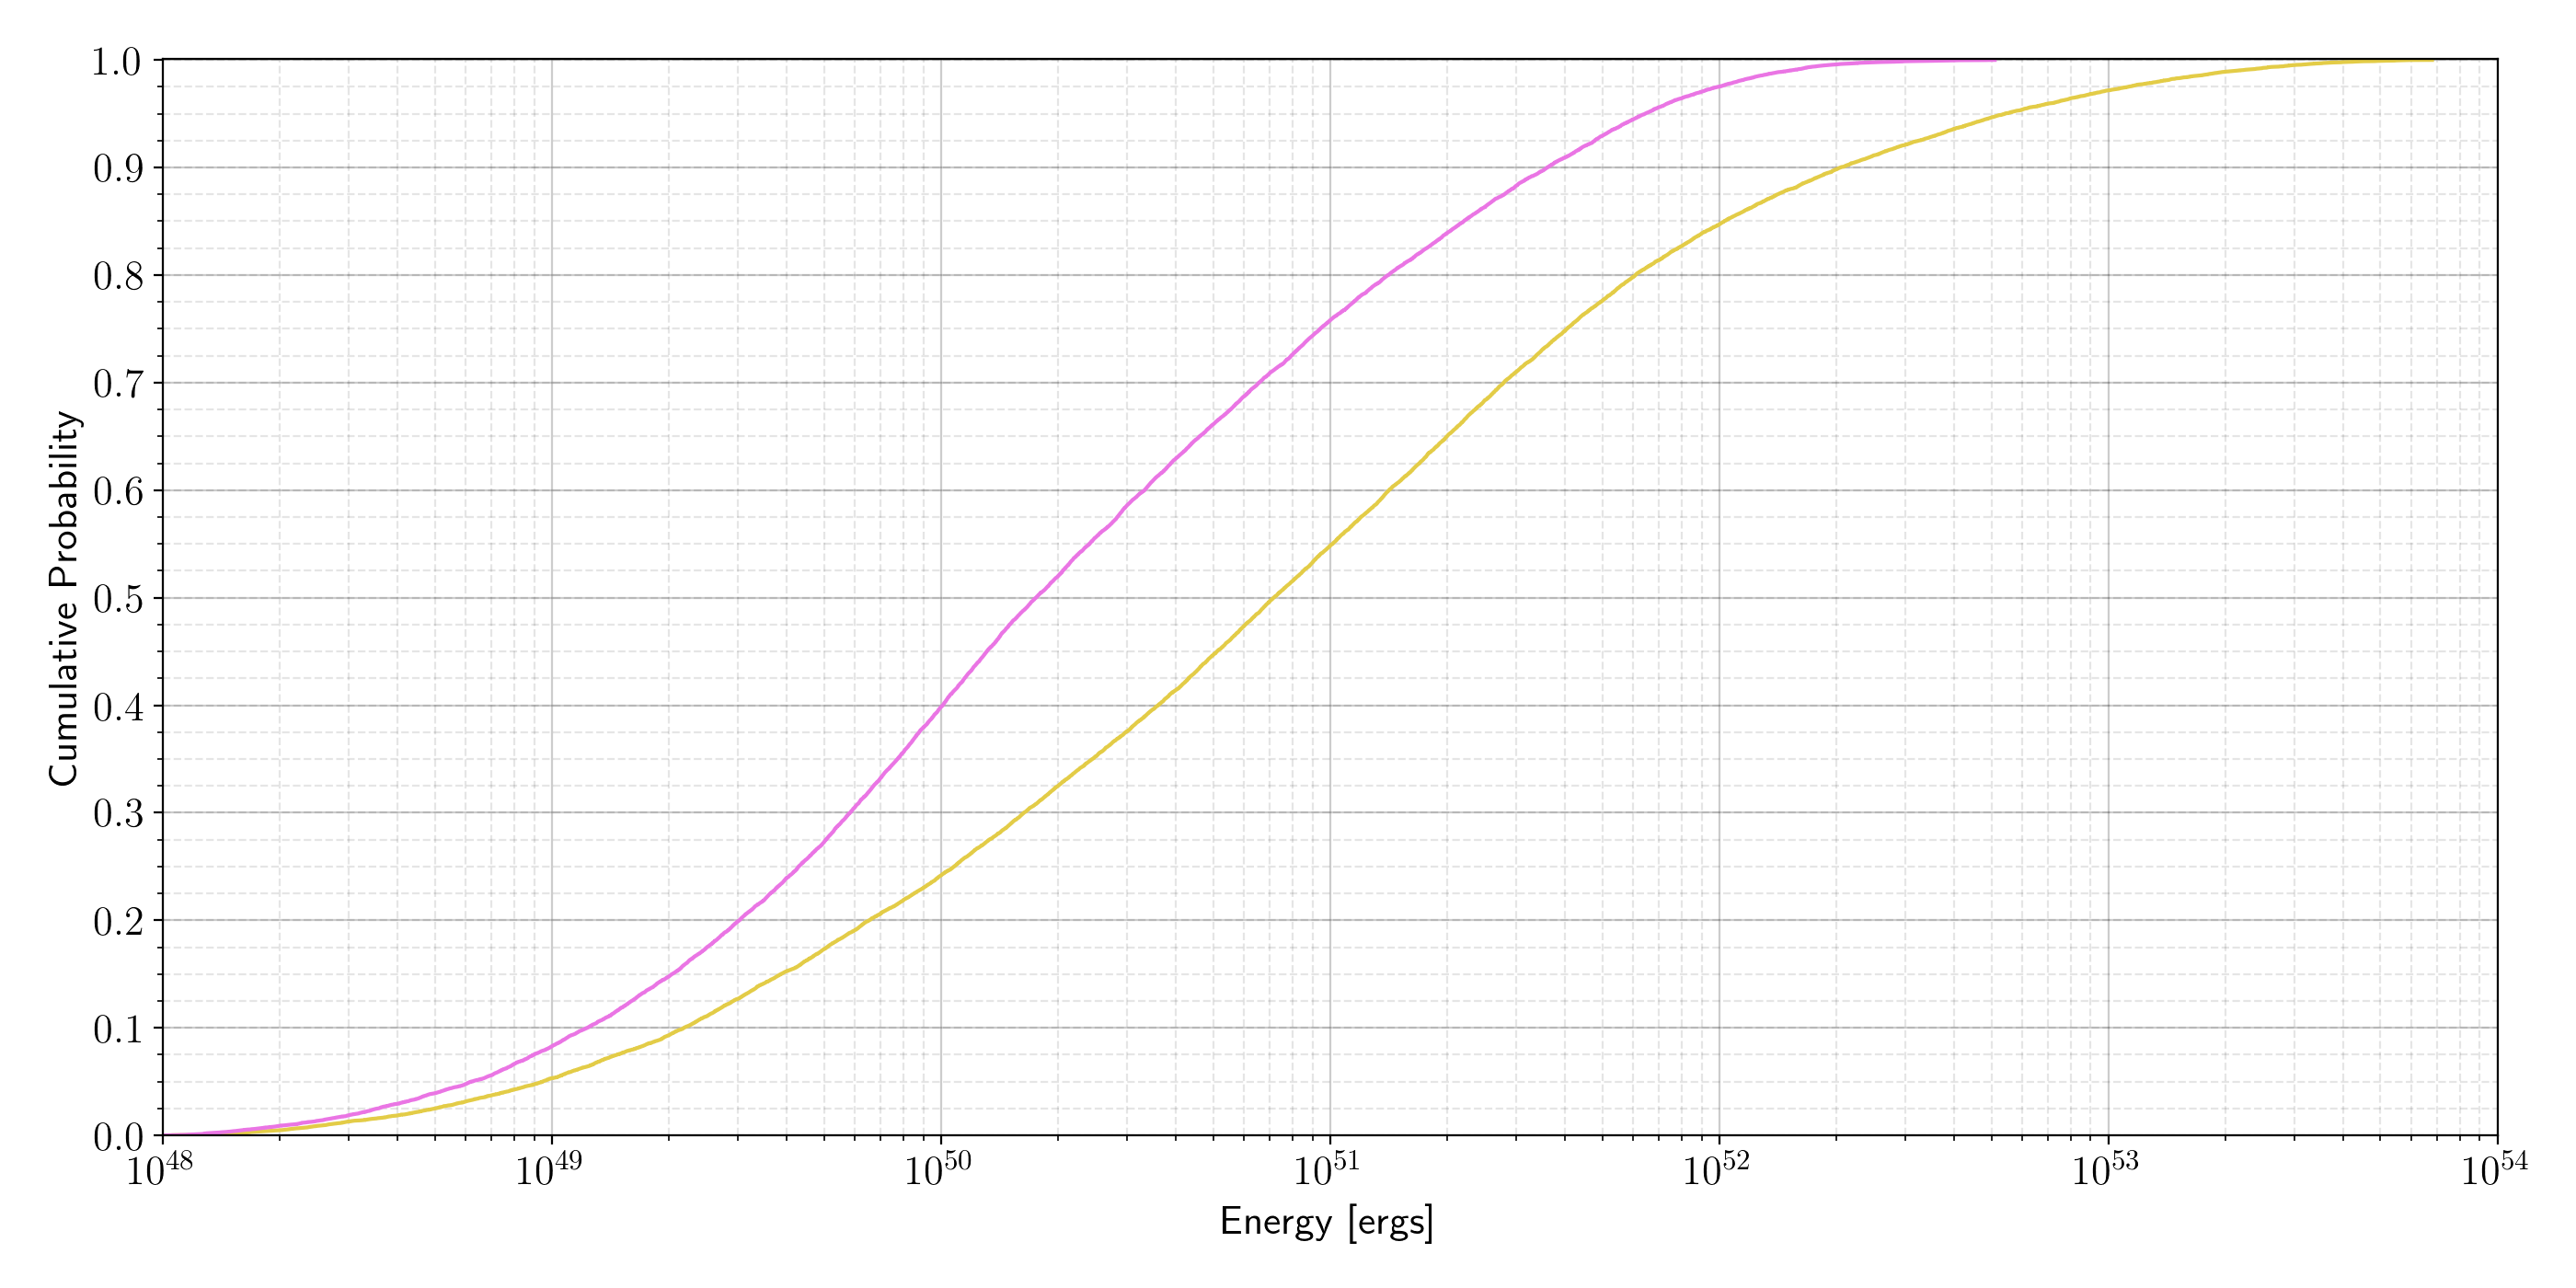
\includegraphics[width=\columnwidth]{uniform_narrow_f0_energy_cumulative_posterior_probability}
\caption{The cumulative probability for the energy dissipated through nonlinear tides from the prior probability distribution (yellow), and from the posterior probability distribution (dark pink) at the inner-most stable circular orbit, $f_\mathrm{ISCO}$. These data are from the analysis with a uniform prior on the mass, for $15 \leq f_0 \leq 100$~Hz range, and $\delta \phi$ $>$ 0.1 radians constraint. This is for the prior distribution with For reference, gravitational waves for neutron stars of the estimated mass range of GW170817 carry $\gtrsim \, 10^{53}$~ergs of energy. Note that the inferred energy dissipation through nonlinear tides has decreased from the prior belief of plausible energy dissipation through nonlinear tides.
}
\label{fig:uniform_f0_small_NL_energy}
\end{figure}

We also examine the leading order estimated energy dissipated through nonlinear tides, see Fig.~\ref{fig:uniform_f0_small_NL_energy}. Here we examine the energy dissipated for a uniform prior on the mass, with $15 \leq f_0 \leq 100$~Hz, with a $\delta \phi$ $>$ 0.1 radians constraint. In our analysis, the $90^{\mathrm{th}}$ percentile of the estimated energy dissipated through nonlinear tides from our prior distribution is approximately $2 \times 10^{52}$~ergs at the terminating frequency of the TaylorF2 waveform, $f_\mathrm{ISCO}$. This is approximately $10 \%$ of the estimated energy radiated by gravitational waves by neutron stars of the estimated mass range of GW170817. Our analysis finds the energy dissipated through nonlinear tides at the $90\%$ posterior credible level is $3.6 \times 10^{51}$~ergs. We find our $90\%$ posterior credible level to be comparable to the $90\%$ posterior credible level of $2.7 \times 10^{51}$~ergs in~\cite{abbott2019constraining}. Samples from our posterior distribution that have dissipation energies greater than $10^{52}$~ergs tend to come from large $A$, $n \sim 4/3$, and low $f_0$, as well as $A \sim 10^{-7}$ and $1.6 \lesssim n < 3.0$.

\section{Discussion}
In this paper, we have used the GW170817 signal and the model of~\cite{Essick:2016tkn} to look for evidence of nonlinear tides from $p$-$g$ mode coupling during the inspiral~\citep{Weinberg:2013pbi,Weinberg:2015pxa,Zhou:2018tvc}. Our Bayes factor of unity yields an inconclusive result on whether nonlinear tides are favored or disfavored in GW170817. A closer examination of the posterior distribution lead us to conclude that either nonlinear tides are not measurable in GW170817, because they cause very small phase shifts to waveform, or the nonlinear tides must enter the waveform by being degenerate with the other intrinsic parameters of GW170817. A further investigation of the parameter space also permitted us to constrain that nonlinear tidal waveforms from a $p$-$g$ mode instability with $<98.5 \%$ overlap with standard waveforms can be ruled out at a Bayes factor of $>30$.

In principle, one could improve our analysis by separately parameterizing the amplitude, turn-on frequency, and frequency evolution for each star as in~\cite{abbott2019constraining}. However, we find our results to be consistent with~\cite{abbott2019constraining}, and so we do not expect these to affect the main conclusion of our paper. Future studies may also examine higher order post-Newtonian contributions from the $p$-$g$ mode instability.

Improved knowledge of the interior dynamics of neutron star cores and crusts, and its interaction with neutron star magnetic fields may yield a better parametrized model regarding $p$-$g$ mode instabilities~\citep{Weinberg:2015pxa}. Nonlinear tides are poorly understood and the contribution from other stellar oscillation modes may yet contribute to a more accurate picture of the interior dynamics of neutron stars~\citep{Andersson:2017iav}. Future LIGO-Virgo Collaboration observing runs will likely provide new observations of binary neutron star mergers~\citep{Abbott:2016ymx,ligo2018gwtc}. With the expected improvements in detector sensitivity, it may be possible to find evidence for a measurable $p$-$g$ mode instability in coalescing binary neutron stars in the future.

%% If you wish to include an acknowledgments section in your paper,
%% separate it off from the body of the text using the \acknowledgments
%% command.

\acknowledgments

We thank Reed Essick, and Nevin Weinberg for pointing out errors in our Bayes factor calculation in an earlier draft of this paper~\citep{Essick:2018wvj}. We  thank Chaitanya Afle, Soumi De, and Daniel Finstad for helpful discussions. We thank Alex Nitz for writing the initial version of the code for nonlinear tides in PyCBC. The authors were supported by the National Science Foundation grant PHY-1707954. Computational work was supported by Syracuse University and National Science Foundation grant OAC-1541396. This research has made use of data obtained from the Gravitational Wave Open Science Center (\url{https://www.gw-openscience.org/about/}).


\software{PyCBC Inference \citep{alex_nitz_2018_1208115,biwer2019pycbc},  
          emcee \citep{emcee,vousden:2016}, 
          LIGO Algorithm Library \citep{lal},
          Matplotlib \citep{Hunter:2007},
          Scipy \citep{scipy}
          }


\bibliography{references}

\begin{figure}[th]
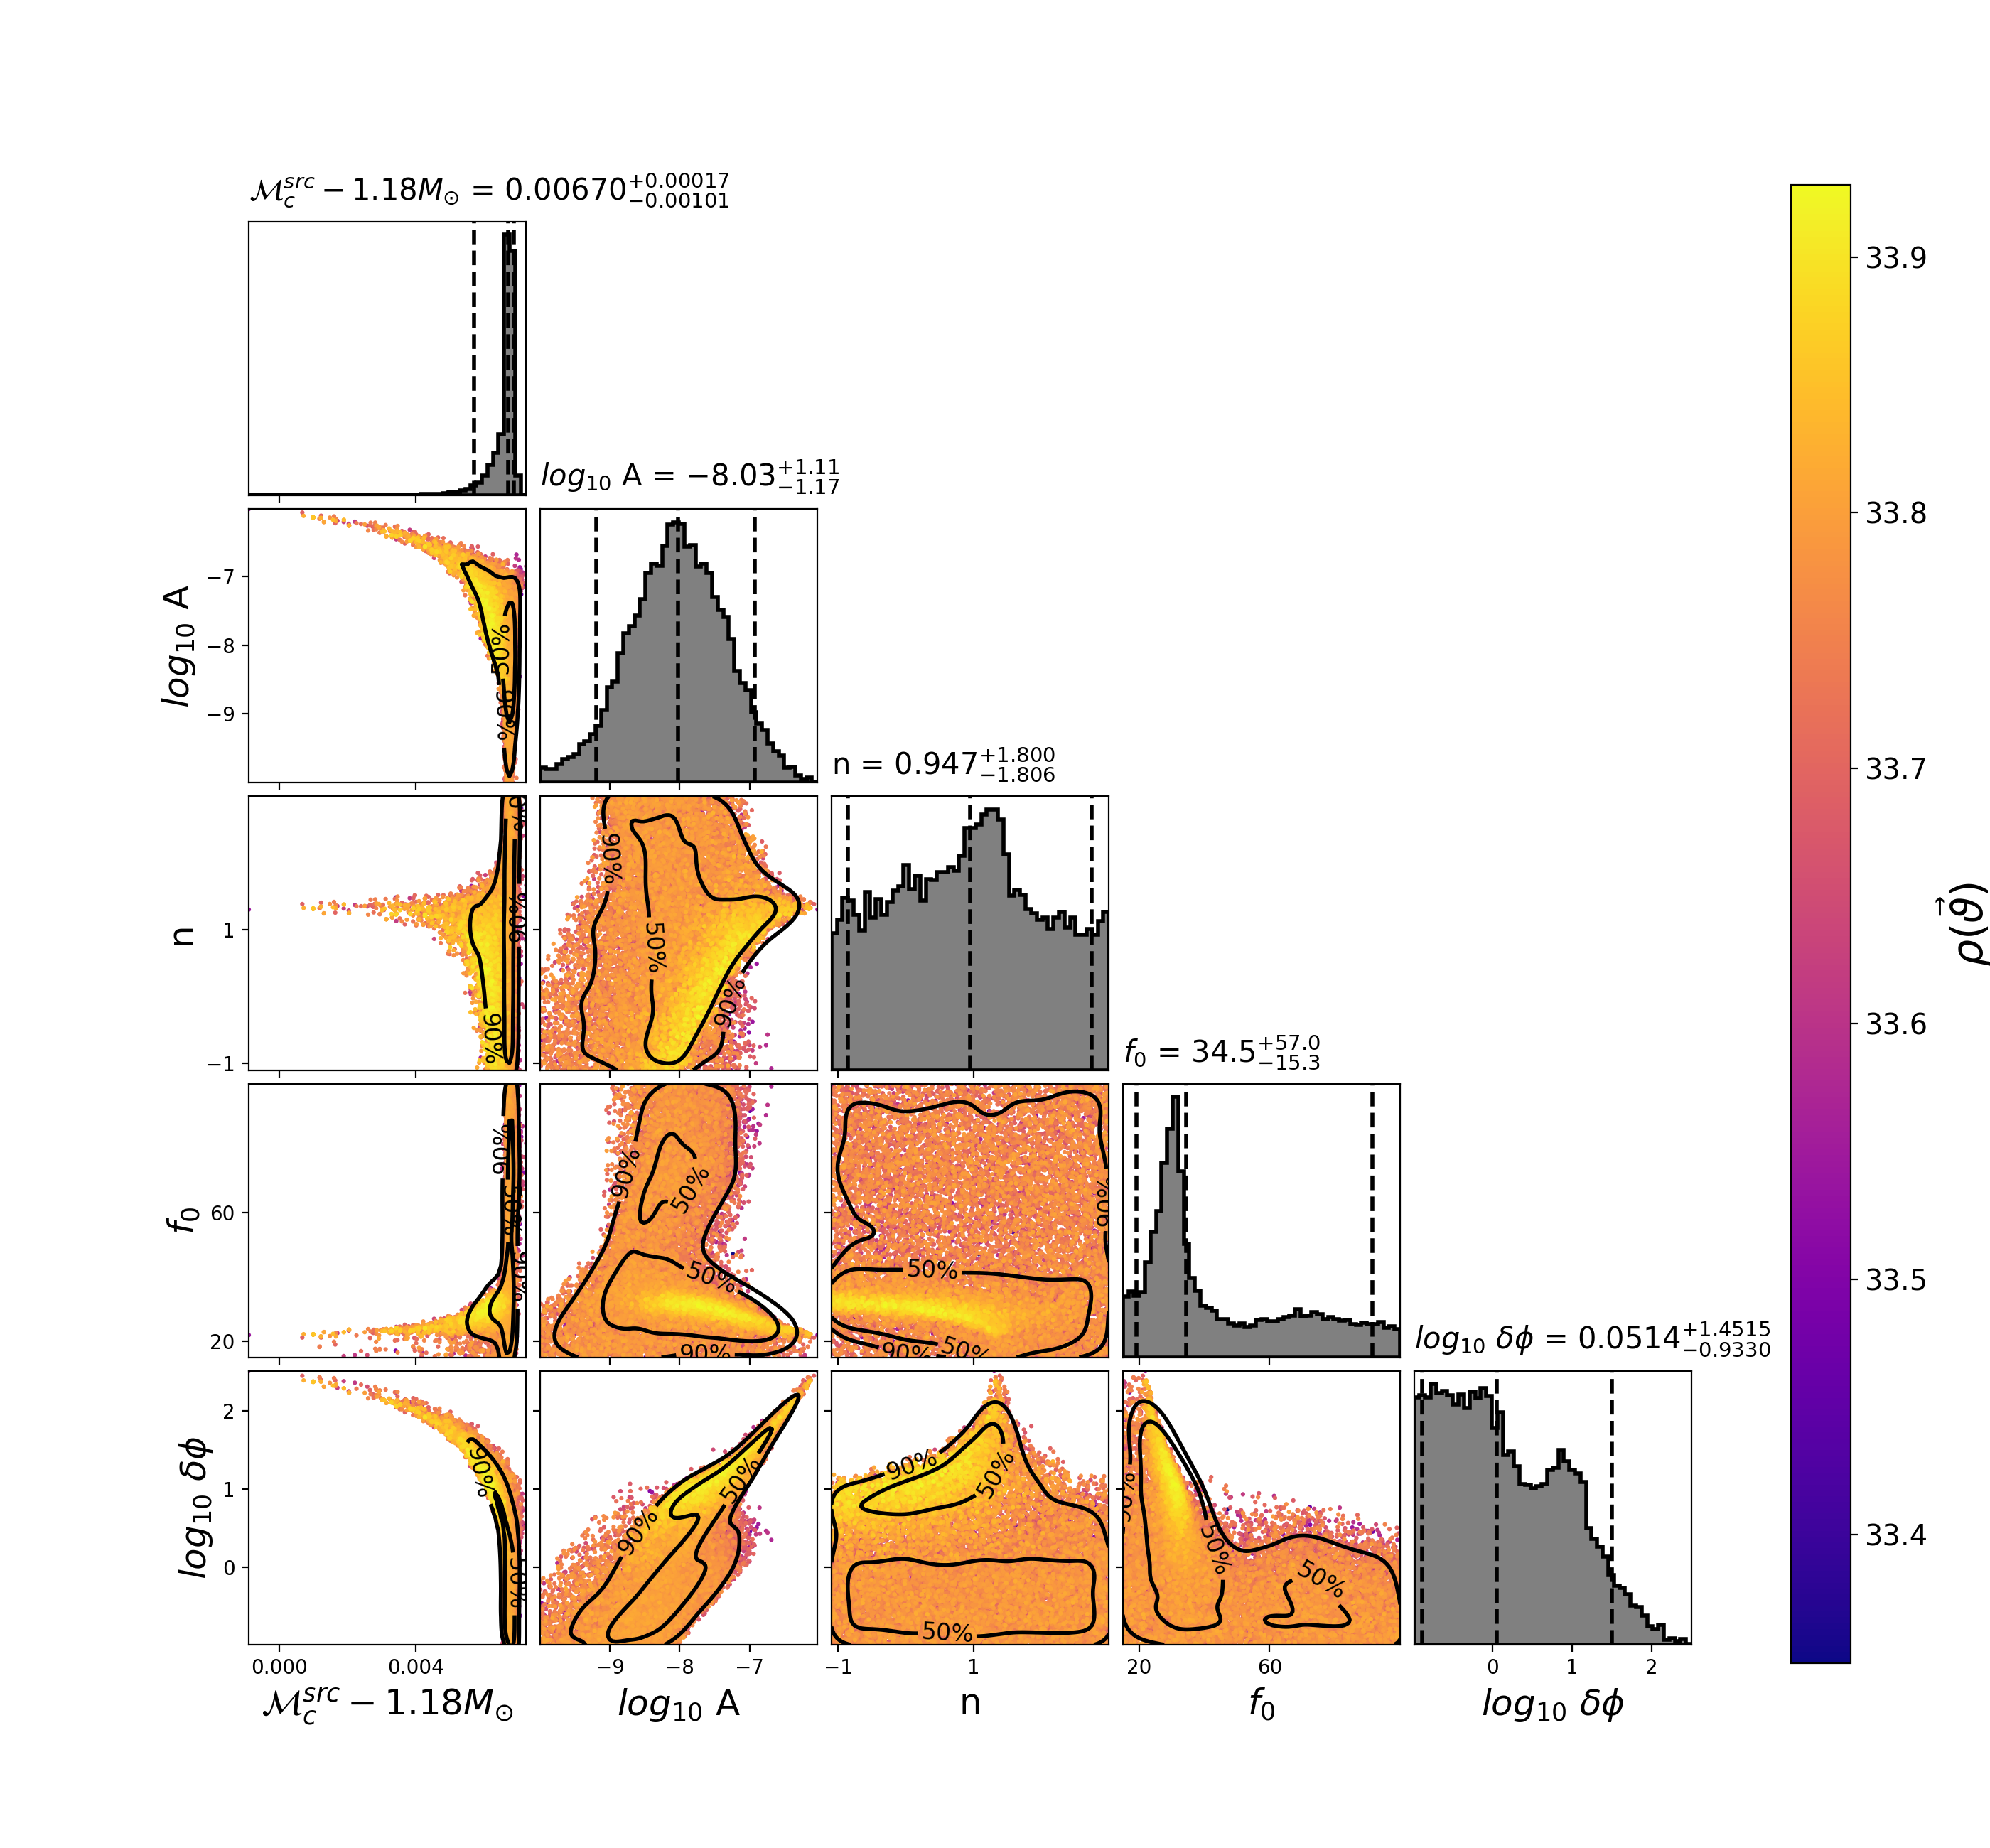
\includegraphics[width=\columnwidth]{combined_uni_dphi_cut_combined}
\caption{The marginalized posterior distributions for the uniform mass prior and a $f_0$ restricted to the range $15$ and $100$~Hz. The vertical lines on the marginalized histograms display the $5$th, $50$th, and $95$th percentiles of the posteriors. The three-detector network signal-to-noise ratio for each sample is given on the color-bar. The posterior scatter plots show 50\% and 90\% credible interval contours. The posteriors on $n$ is peaked $n \lesssim 4/3$ and for values of $f_0$ close to the lower end of the detector's low frequency sensitivity. In this region of parameters space, the effect of nonlinear tides is degenerate with chirp mass, causing a secondary peak in the chirp mass posterior. It can be seen from the $\delta\phi$--$\mathcal{M}$ plot (lower left) that large phase shifts due to nonlinear tides are due to points in parameter space where a value of chirp mass can be found that compensates for the phase shift of the nonlinear tides. These are the combined posteriors from $9$ runs. It is notable that the the peaks in the $f_0$ posterior, at $f_0 \approx 30$~Hz and $f_0 \approx 70$~Hz seem to be reversed from those in Fig 2. of \citep{abbott2019constraining}. Note that the marginalized posterior for $A$ is diminished for $A < 10^{-8}$ due to the $\delta \phi$ prior constraint.
}
\label{fig:uniform_f0_small}
\end{figure}
